\begin{document}

\section{Results}

\subsection{Training Neural Network}


\subsubsection{Experiment 1}

    
    
    The below graph aims to show the scalability of Apache Spark and Analytics Zoo for Big Data Operations. The neural network model was trained using NN Frames, an API on Analytics Zoo. The Spark Program was in local mode (not distributed as only single node was used) using an Intel I7 8th gen CPU (with 4/4 cores used), batch size of 2048 and trained for 50 epochs. The model was trained separately using datasets of 3 different sizes. Dataset-1 has only 80000 records, Dataset-2 has 170000 records and Dataset-3 has 240000 records. Proccessing time per record was almost identical, with all results being within 10\% of each other. Due to architecture issues, the training program could not be deployed on the cluster.  
    
    \begin{figure}[H]
          
          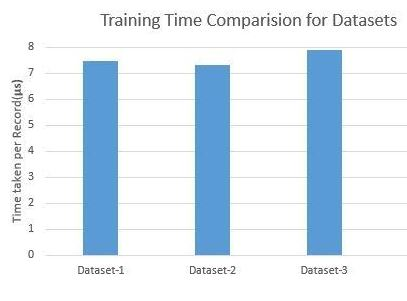
\includegraphics[scale=0.8]{images/Exp1.JPG}
          \caption{Training on Local PC using Different Datasets}
          \label{fig:Exp1}
              
    \end{figure}

\subsubsection{Experiment 2 }
    
    
    
    A Keras model was created (using a Tensorflow backend) using Azure Notebooks  and exported in HDF5, the standard Tensorflow format. The model was then imported by training programs coded using Analytics Zoo and DL4J and run using local mode on the different datasets (used in previous experiment).
    
    \begin{figure}[H]
          
          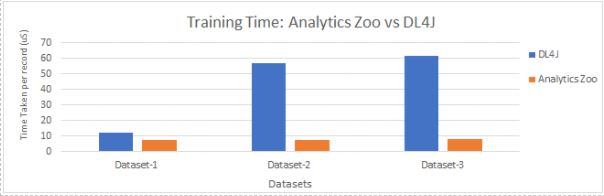
\includegraphics[scale=0.8]{images/Exp2.JPG}
          \caption{Training on Analytics Zoo vs DL4J in Local Mode }
          \label{fig:Exp2}
              
    \end{figure}
    
    The network training using Analytics Zoo was found to be faster than DL4J for all datasets. Using dataset 2 and 3 it is observed that Analytics Zoo was more than 10 times faster compared to DL4J. This shows that Analytics Zoo is more scalable for Big Data operations as it retains its performance when the dataset size increases while DL4J performance suffers. 
    
\subsection{Inference using Software Program}

    This experiment shows the limitations of using a distributed system. Due to lack of a sufficiently large dataset, this experiment limited the memory of each executor of the RPi Cluster on the A-Fog to 1GB. It was found that the distributed system performed faster when the memory per executor was lower. This is due to the fact that the distributed system incurs a communication latency which does not exist when using a single Raspberry Pi. The performance benefit of the distributed system is significant when there is a big dataset (modelled by limiting memory) while it will be outweighed by latency of communication for smaller datasets.
    
    \begin{figure}[H]
          
          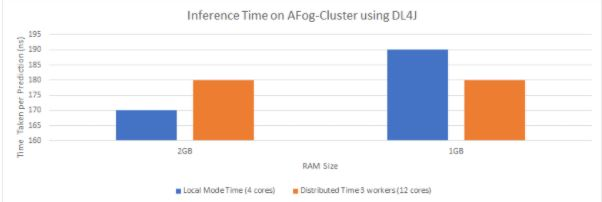
\includegraphics[scale=0.8]{images/Exp3.JPG}
          \caption{ Software Inference Time for Local vs Distributed Mode  }
          \label{fig:Exp3}
              
    \end{figure}
    
\subsection{Inference: Software VS Hardware}
    This experiment compares the processing time per record between a single Raspberry Pi (software) and the Pynq board (hardware). For smaller batch sizes, the software computes inference faster than the Pynq board. This is because the the communication overheads in the Pynq board affect the results for small batch sizes. As the batch size increases, this overhead is not as significant and it can be seen that  hardware solution outperforms the software. 
    
    \begin{figure}[H]
          
          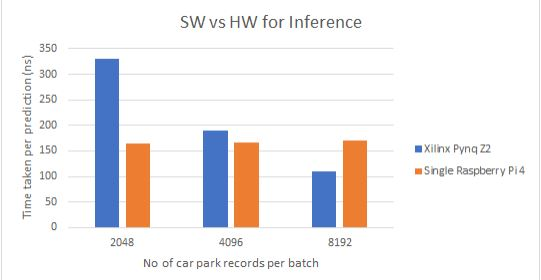
\includegraphics[scale=0.8]{images/Exp4.JPG}
          \caption{Inference using SW Program on Raspberry Pi 4 or Hardware Block on Pynq Board}
          \label{fig:Exp4}
              
    \end{figure}


%%%%
% DISCUSSION/FUTURE WORK
%
%%%%

\section{Discussion/Future Work}

The findings clearly show that Analytics Zoo is much faster than DL4J when training Neural Networks on the Host PC. The primary reason for this is the different libraries used for mathematical operations. Analytics Zoo is a tool developed by Intel and only supports a library called Intel Math Kernel Library (MKL), while DL4J uses OpenBLAS as its default library. OpenBLAS has been benchmarked and is on average 5 times slower [dl4j docs]. DL4J can also be configured with different backend libraries but this was not trialed as distributed training did not work due to dependency issues. The issue identified when developing this platform was that Intel MKL only supports intel processor architectures. This means that Analytics Zoo cannot be run on the RPi cluster, due to Raspberry Pi 4 having an ARM proccesor which is not supported.  A potential solution to this was using an open source fork of Intel MKL which has support for ARM64 architecture. OpenDNN [https://github.com/oneapi-src/oneDNN] is one such solution, however it only provides experimental support and is not verified to be functional. The additional problem with using such external dependencies is lack of support in the future as these are fully open source solutions with no company funding. Using external libaries also adds to the developmental overhead, as libraries like Analytics Zoo would require source code to be edited in order to configure them to work with the alternative library rather than Intel MKL.   

A viable solution found to this problem was to modify the A-Fog cluster. The RPi cluster consists of raspberry pi 4 devices which have ARM64 architecture, which is prevalent in low cost embedded devices [https://cacm.acm.org/magazines/2011/5/107684-an-interview-with-steve-furber/fulltext ].  

This cluster can be replaced by a device where the processor uses an x86 architecture. Some devices are explored below. 

 

 ODYSSEY – X86J4105 is one such solution manufactured by Seed Studio. It contains an Intel Celeron processor, which has an x86 architecture. The device supports windows and linux operating systems and contains 8GB of RAM along with the desired peripherals such as ethernet,wifi,sim card and SATA (for external storage).  It is designed to be an edge-computing device and also contains an ARM co-processor. Cost is a disadvantage however, the device retails at around \$200, which is considered expensive for a Single Board Computer. 

[https://www.seeedstudio.com/ODYSSEY-X86J4105864-p-4447.html] 

A solution that is lower cost is Latte Panda which retails from \$90. It contains an Intel Atom processor, which contains x86 architecture but is not as powerful as the Odyssey. This device also features support for windows and linux operating systems but only contains from 2GB-4GB of RAM along with the device. It features similar peripherals to the Odyssey but does not contain a sim card or SATA.  An ATMega co-proccesor is also present in this board. [https://www.lattepanda.com/products/3.html] 




\end{document}

